\documentclass[
  captions=tableheading,
  bibliography=totoc, 
  titepage=firstiscover,
]{scrartcl}

\usepackage{blindtext} %neuer input

\usepackage{longtable} % Tabellen über mehrere Seiten

\usepackage[utf8]{inputenc} %neuer input

\usepackage{scrhack}

\usepackage[aux]{rerunfilecheck} %Warnung falls nochmal kompiliert werden muss

\usepackage{fontspec} %Fonteinstellungen

\recalctypearea{}

\usepackage[main=ngerman]{babel} %deutsche Spracheinstellung

\usepackage{ragged2e} %neuer input

\usepackage{amsmath, nccmath}

\usepackage{amssymb} %viele mathe Symbole

\usepackage{mathtools} %Erweiterungen für amsmath


\DeclarePairedDelimiter{\abs}{\lvert}{\rvert}
\DeclarePairedDelimiter{\norm}{\lVert}{\rVert}

\DeclarePairedDelimiter{\bra}{\langle}{\rvert}
\DeclarePairedDelimiter{\ket}{\lvert}{\rangle}

\DeclarePairedDelimiterX{\braket}[2]{\langle}{\rangle}{
#1 \delimsize| #2
}

\NewDocumentCommand \dif {m}
{
\mathinner{\symup{d} #1}
}


\usepackage[
  math-style=ISO,
  bold-style=ISO,
  sans-style=italic,
  nabla=upright,
  partial=upright,
  warnings-off={
    mathtools-colon,
    mathtools-overbracket,
  },
]{unicode-math}

\setmathfont{Latin Modern Math}
\setmathfont{XITS Math}[range={scr, bfscr}]
\setmathfont{XITS Math}[range={cal, bfcal}, StylisticSet=1]


\usepackage[
  locale=DE,
  separate-uncertainty=true,
  per-mode=reciprocal,
  output-decimal-marker={,},
]{siunitx}

\usepackage[autostyle]{csquotes} %richtige Anführungszeichen

\usepackage{xfrac}

\usepackage{float}

\floatplacement{figure}{htbp}

\floatplacement{table}{htbp}

\usepackage[ %floats innerhalb einer section halten
  section,   %floats innerhalb er section halten
  below,     %unterhalb der Section aber auf der selben Seite ist ok
]{placeins}

\usepackage[
  labelfont=bf,
  font=small,
  width=0.9\textwidth,
]{caption}

\usepackage{subcaption} %subfigure, subtable, subref

\usepackage{graphicx}

\usepackage{grffile}

\usepackage{booktabs}

\usepackage{microtype} %Verbesserungen am Schriftbild

\usepackage[
backend=biber,
]{biblatex}

\addbibresource{../lit.bib}

\usepackage[ %Hyperlinks im Dokument
  german,
  unicode,
  pdfusetitle,
  pdfcreator={},
  pdfproducer={},
]{hyperref}

\usepackage{bookmark}

\usepackage[shortcuts]{extdash}

%\usepackage{warpcol}


\begin{document}
    \title{Physik IV Übungsblatt 2}
    \author{  
    Tobias Rücker\\
    \texorpdfstring{\href{mailto:tobias.ruecker@tu-dortmund.de}{tobias.ruecker@tu-dortmund.de}
    \and}{,} 
    Paul Störbrock\\
    \texorpdfstring{\href{mailto:paul.stoerbrock@tu-dortmund.de}{paul.stoerbrock@tu-dortmund.de}}{}
    }
\maketitle
\center{\Large Abgabegruppe: \textbf{4 H}}
\thispagestyle{empty}

\newpage
\tableofcontents
\thispagestyle{empty}
\newpage

\setcounter{page}{1}


\section{Aufagabe 1}

\begin{figure}[H]
    \centering
    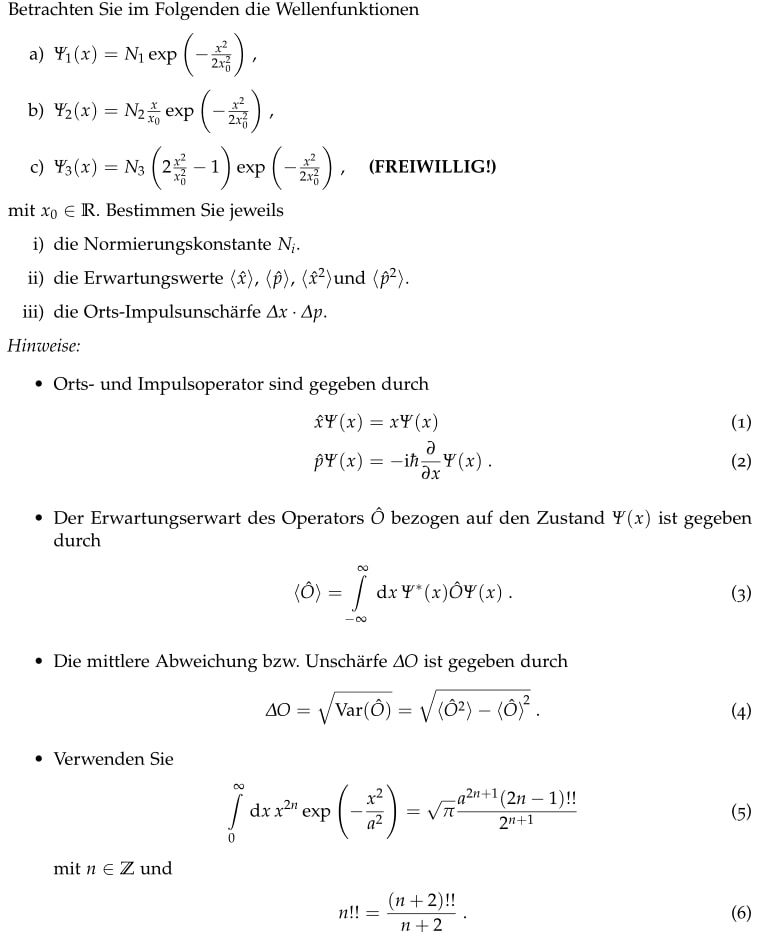
\includegraphics[width=0.75\textwidth]{images/Aufgabe_1.jpg}
    \label{fig:1}
\end{figure}

\subsection{a)}

\subsubsection{i)}

    \begin{align*}
        \Psi_1(x) &= N_1 \cdot exp \left(- \frac{x^2}{2x_0^2} \right)\\
        \int_{-\infty}^{\infty} \abs{\Psi_1 (x)}^2 \; \mathrm{d}x &\stackrel{!}{=} 1\\
        \int_{-\infty}^{\infty} \abs{N_1 \cdot exp \left(-\frac{x^2}{2x_0^2} \right)} ^2 \; \mathrm{d}x &= 1 \nonumber\\
        \abs{N_1}^2 \int_{-\infty}^{\infty} exp \left(-\frac{x^2}{2x_0^2} \right) \; \mathrm{d}x &= 1 \nonumber\\
        u = \frac{x}{x_0} \qquad \rightarrow \qquad \frac{\mathrm{d}u}{\mathrm{d}x} &= \frac{1}{x_0} 
        \qquad \Leftrightarrow \qquad \mathrm{d}u = \frac{1}{x_0} \mathrm{d}x \nonumber\\
        \abs{N_1}^2 \int_{-\infty}^{\infty} x_0 \cdot exp \left(-\frac{x^2}{2x_0^2} \right) \; \mathrm{d}u &= 1 \nonumber\\
        \abs{N_1}^2 \cdot x_0 \cdot \sqrt{\pi} &= 1 \nonumber\\
        \abs{N_1} &= \pm \sqrt{\frac{1}{\sqrt{\pi}x_0}} \qquad \qquad \qquad (A)
    \end{align*}

\subsubsection{ii)}

    \begin{align*}
        \hat{x} \Psi &= x \Psi\\
        \langle \hat{x} \rangle &= \int_{-\infty}^{\infty} \abs{N_1}^2 exp \left(- \frac{x^2}{2x_0^2}\right) \; \mathrm{d}x\\
        u = \frac{x}{x_0} \qquad \rightarrow \qquad \frac{\mathrm{d}u}{\mathrm{d}x} &= \frac{1}{x_0} 
        \qquad \Leftrightarrow \qquad \mathrm{d}u = \frac{1}{x_0} \mathrm{d}x \nonumber\\
        &= - \int_{-\infty}^{\infty} x_0 \cdot \abs{N_1}^2 \cdot exp \left(- u^2 \right) \; \mathrm{d}u \nonumber\\
        &= x_0^2 \abs{N_1}^2 \cdot \frac{1}{2} \left[ e^{- u^2} \right]_{-\infty}^{\infty} \nonumber\\
        \langle \hat{x} \rangle_{\Psi_1} &= 0 \qquad \qquad \qquad (B)\\
        \hat{p} \Psi_1 &= -i \hbar \frac{\partial}{\partial x} \Psi_1\\
        &= i \hbar \abs{N_1} \frac{x}{x_0^2} \cdot exp \left(-\frac{x^2}{2x_0^2} \right) \nonumber\\
        \langle \hat{p} \rangle &= \int_{-\infty}^{\infty} \Psi_1^* \hat{p} \Psi_1 \; \mathrm{d}x\\
        &= \int_{-\infty}^{\infty} \abs{N_1}^2 exp \left( -\frac{x^2}{2x_0^2} \right) \cdot i \hbar \frac{x}{x_0^2} exp \left(- \frac{x^2}{2x_0^2} \right)
        \; \mathrm{d}x \nonumber\\
        &= i \hbar \abs{N_1}^2 \int_{-\infty}^{\infty} x \cdot exp \left(- \frac{x^2}{2x_0^2} \right) \; \mathrm{d}x \nonumber\\
        &= - \frac{1}{2} i \hbar \abs{N_1}^2 x_0 \left[ exp \left(- u^2 \right) \right]_{-\infty}^{\infty} \nonumber\\
        \langle \hat{p} \rangle_{\Psi_1} &= 0 \qquad \qquad \qquad (C)\\
        \langle \hat{x}^2 \rangle &= \int_{-\infty}^{\infty} \Psi_1^2(x) x^2 \; \mathrm{d}x\\
        &= \int_{-\infty}^{\infty} \abs{N_1}^2 x^2 exp \left(- \frac{x^2}{2x_0^2} \right) \; \mathrm{d}x \nonumber
        \intertext{\flushleft{Da\;}\justifying die Gaußkurve symmetrisch ist, folgt:
        }
        &= 2 \cdot \int_{0}^{\infty} \abs{N_1}^2 x^2 exp \left(- \frac{x^2}{2x_0^2} \right) \; \mathrm{d}x \nonumber\\
        &\stackrel{Blatt\;(5)}{=} 2 \abs{N_1}^2 \cdot \sqrt{\pi} \frac{x_0^3(1)!!}{2^2} \qquad \text{für $n = 1$} \nonumber\\
        &= 2 \abs{N_1}^2 \cdot \sqrt{\pi} \frac{x_0^3}{8} \qquad \qquad \qquad (D)\\
        \langle \hat{x}^2 \rangle_{\Psi_1} &\stackrel{(A)}{=} \frac{1}{2} \cdot x_0^2\\
        \langle \hat{p}^2 \rangle &= \int_{-\infty}^{\infty} \abs{N_1}^2 exp \left(- \frac{x^2}{2x_0^2} \right) (-\hbar) \frac{\partial ^2}{\partial x^2} 
        \abs{N_1} \cdot exp \left(- \frac{x^2}{2x_0^2} \right) \; \mathrm{d}x\\
        &= - \hbar \abs{N_1}^2 \int_{-\infty}^{\infty} exp \left(- \frac{x^2}{2x_0^2} \right) \frac{\partial}{\partial x} \left( -\frac{x}{x_0^2} 
        \right) exp \left(- \frac{x^2}{2x_0^2} \right) \; \mathrm{d}x \nonumber\\
        &= - \hbar \abs{N_1}^2 \int_{-\infty}^{\infty} exp \left(- \frac{x^2}{2x_0^2} \right) \left( -\frac{1}{x_0^2} + \frac{x^2}{x_0^4} \right) 
        exp \left(- \frac{x^2}{2x_0^2} \right) \; \mathrm{d}x \nonumber\\
        &\stackrel{!}{=} -2 \hbar \abs{N_1}^2 \int_{0}^{\infty} \left( -\frac{1}{x_0^2} + \frac{x^2}{x_0^4} \right) exp \left(- \frac{x^2}{2x_0^2}
        \right) \; \mathrm{d}x \nonumber\\
        &= -2 \hbar \abs{N_1}^2 \int_{0}^{\infty} \left( -\frac{1}{x_0^2} \sqrt{\pi} \frac{x_0}{2} + \frac{1}{x_0^4} \sqrt{\pi} \frac{x_0^3}{2^2}
        \right) \nonumber\\
        &= -2 \hbar \abs{N_1}^2 \left( -\frac{1}{4} \frac{\sqrt{\pi}}{x_0} \right) = \frac{1}{2} \sqrt{\pi} \hbar \frac{\abs{N_1}^2}{x_0} \nonumber\\
        \langle \hat{p}^2 \rangle_{\Psi_1} &\stackrel{(A)}{=} \frac{1}{2} \frac{\hbar}{x_0^2}
    \end{align*}

\subsubsection{iii)}

    \begin{align*}
        \Delta x &= \sqrt{\langle \hat{x}^2 \rangle - \langle \hat{x} \rangle^2}\\
        &= \sqrt{\frac{x_0^2}{2}} = \frac{\abs{x_0}}{\sqrt{2}}\\
        \Delta p &= \sqrt{\langle \hat{p}^2 \rangle - \langle \hat{p} \rangle^2}\\
        &= \sqrt{\frac{\hbar}{2 x_0^2}}\\
        \Delta x \cdot \Delta p &= \frac{\abs{x_0}}{\sqrt{2}} \cdot \sqrt{\frac{\hbar}{2 x_0^2}}
        = \frac{\hbar}{2}
    \end{align*}

\subsection{b)}

\begin{align}
    \Psi_2 (x)=N_2 \frac{x}{x_0} \exp{-\frac{x^2}{2x_0^2}}
\end{align}

\subsubsection{i)}

\begin{align}
    &\int_{-\infty}^{\infty}\,dx\, \abs{N_2\frac{x}{x_0}\exp\left(-\frac{x^2}{2x_0^2}\right)}^2=1\\
    &\abs{N_2}^2 \int_{-\infty}^{\infty}\,dx\, \abs{\frac{x}{x_0}\exp\left(-\frac{x^2}{2x_0^2}\right)}^2=1\\
    &\abs{N_2}^2 \left(\int_0^{\infty}\,dx\,\left(\frac{x}{x_0}\exp\left(-\frac{x^2}{2x_0^2}\right)\right)^2+ \int_{-\infty}^0\,dx\,\left(-\frac{x}{x_0} \exp\left(-\frac{x^2}{2x_0^2}\right)\right)^2 \right)=1\\
    &2 \abs{N_2}^2 \int_0^{\infty}\,dx\, \frac{x^2}{x_0^2} \exp\left(-\frac{x^2}{x_0^2}\right)=1\\
    &2 \abs{N_2}^2 \left(\sqrt{\pi} \frac{1}{x_0^2} \frac{x_0^3}{2^2}\right)=1\\
    &\abs{N_2}^2=\frac{2}{x_0\sqrt{\pi}}\\
    &\abs{N_2}= \pm \sqrt{\frac{2}{x_0\sqrt{\pi}}}
\end{align}

\subsubsection{ii)}

\begin{align}
    <\hat x > &= \int_{-\infty}^{\infty}\,dx\, \Psi _2^* \hat x \Psi _2\\
    &= \int_{-\infty}^{\infty}\,dx\, x\cdot  \abs{N_2}^2 \frac{x^2}{x_0^2}\exp(-\frac{x^2}{x_0^2})\\
    &=\int_{-\infty}^{\infty}\,dx\, \underbrace{\underbrace{\frac{x^3}{x_0^2}}_{\text{ungerade Fkt}} \underbrace{\exp(-\frac{x^2}{x_0^2})}_{\text{gerade Fkt}}}_{\text{ungerade Fkt}}\\
    \intertext{
        $\Rightarrow $ Integral $\;I \in (-\infty,\infty) \; 0\; $ ist
    }
    <\hat x >_{\Psi_2}&=0
\end{align}

\begin{align}
    <\hat x ^2> &= \int_{-\infty}^{\infty}\,dx\, \abs{N_2}^2 x^2 \frac{x^2}{x_0^2} \exp\left(-\frac{x^2}{x_0^2}\right)\\
    &=\frac{1}{x_0^2} \abs{N_2}^2 2 \int_0^{\infty}\,dx\, x^4 \exp\left(-\frac{x^2}{x_0^2}\right)\\
    &=\frac{1}{x_0^2} \abs{N_2}^2 2\sqrt{\pi} \frac{x_0^5(2\cdot2-1)!!}{2^3}\\
    &=\frac{3\sqrt{\pi}}{4}x_0^3 \abs{N_2}^2\\
    <\hat x ^2>_{\Psi _2}&= \frac{3}{2} x_0^2
\end{align}

\begin{align}
    <\hat p > &= \int_{-\infty}^{\infty}\,dx\, \Psi _2^*\hat p \Psi _2\\
    &=\int_{-\infty}^{\infty}\,dx\, N_2^* \frac{x}{x_0} \exp\left(-\frac{x^2}{2x_0^2}\right) (-i\hbar) \frac{\partial}{\partial x}\left(\frac{x}{x_0} N_2 \exp \left(-\frac{x^2}{2x_0^2}\right)\right) \\
    &=(-i\hbar) \frac{\abs{N_2}^2}{x_0^2} \int_{-\infty}^{\infty} \,dx\,x\exp\left(-\frac{x^2}{2x_0^2}\right) \left(1-\frac{x^2}{x_0^2}\right)\exp\left(-\frac{x^2}{2x_0^2}\right)\\
    \intertext{
        $\left(\text{zwei Ungerade Fkt.}\; x \exp\left(-\frac{x^2}{x_0^2} \right) \wedge x^3 \exp\left(-\frac{x^2}{x_0^2} \right) \right)$
    }
    &\Rightarrow <\hat p >_{\Psi _2}=0
\end{align}

\begin{align}
    <\hat p ^2> &= \int_{-\infty}^{\infty}\,dx\, \frac{x}{x_0} N_2^* exp\left(-\frac{x^2}{2x_0^2}\right) (-\hbar^2) \frac{\partial ^2}{\partial x^2}\left(\frac{x}{x_0} N_2 \exp\left(-\frac{x^2}{x_0^2}\right) \right)\\
    &= - \hbar ^2 \frac{\abs{N_2}^2}{x_0^2} \int_{-\infty}^{\infty}\,dx\, x \exp\left(-\frac{x^2}{2x_0^2}\right)\frac{\partial}{\partial x}\left(\left(1-\frac{x^2}{x_0^2}\right)\exp\left(-\frac{x^2}{2x_0^2}\right) \right)\\
    &= - \hbar ^2 \frac{\abs{N_2}^2}{x_0^2} \int_{-\infty}^{\infty}\,dx\, x \exp\left(-\frac{x^2}{2x_0^2}\right)\left(\--\frac{3x}{x_0^2}+\frac{x^3}{x_0^4} \right) \exp\left(-\frac{x^2}{2x_0^2}\right)\\
    &= - \hbar^2 \frac{\abs{N_2}^2}{x_0^4} \int_{-\infty}^{\infty}\,dx\, \left(-3x^2+\frac{x^4}{x_0^2})\exp(-\frac{x^2}{x_0^2}\right)\\
    &= - \hbar^2 \frac{\abs{N_2}^2}{x_0^4} \sqrt{\pi} 2\left(\frac{-3x_0^3}{2^2}+\frac{x_0^5 3!!}{x_0^2\cdot 2^3}\right)\\
    &= \frac{3}{4} \hbar^2 \sqrt{\pi} \abs{N_2}^2 \frac{1}{x_0}\\
    <\hat p ^2 >_{\Psi _2}&=\frac{3}{2} \frac{\hbar ^2}{x_0^2}
\end{align}

\subsubsection{iii)}
\begin{align}
\Delta x&= \sqrt{<\hat x ^2>-<\hat x>^2 }\\
&=\sqrt{3}{2} \abs{x_0}\\
\Delta p &= \sqrt{<\hat p ^2>-<\hat p >^2}\\
&=\sqrt{\frac{3}{2}}\frac{\hbar}{\abs{x_0}}\\
\Delta x \Delta p &= \frac{3}{2} \hbar 
\end{align}

%\subsection{c)}
%
%\subsubsection{i)}
%
%\subsubsection{ii)}
%
%\subsubsection{iii)}



\section{Aufgabe 2}

\begin{figure}[H]
    \centering
    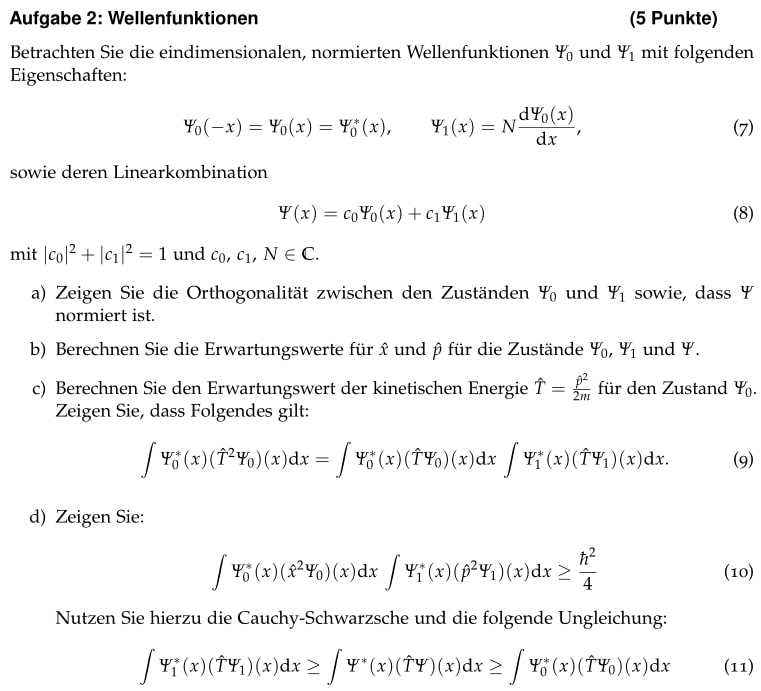
\includegraphics[width=0.75\textwidth]{images/Aufgabe_2.jpg}
    \label{fig:2}
\end{figure}

\subsection{a)}

\flushleft{Beweis\,}\justifying der Orthogonalität zwischen 
$\Psi _1 $ und $\Psi _2 $

Fall $\Psi _0 = \Psi _1$

\begin{align}
    <\Psi _0 , \Psi _0> &= \int_{-\infty}^{\infty} \,dx\, \Psi _0^* \Psi _0\\
    &= \int_{-\infty}^{\infty} \,dx\, \abs{\Psi _0 }^2 \\
    &=1
\end{align}

Beweis, dass $\Psi$ bereits normiert ist:



Fall: $\Psi _0 \ne \Psi _1$

\begin{align}
    <\Psi _0 , \Psi _1> &= \int_{-\infty}^{\infty} \,dx \, \Psi _0^* \cdot \Psi _1\\
    &=\int_{-\infty}^{\infty} \,dx\, \Psi _0 N \frac{\partial \Psi _0 (x)}{\partial x}\\
    &=\int_{-\infty}^{\infty} \,dx\, \frac{N}{2} \frac{\partial}{\partial x}(\Psi _0(x)\cdot \Psi _0(x))\\
    &=\frac{N}{2} \int_{-\infty}^{\infty} \,dx\, \frac{\partial}{\partial x}(\Psi _0(x)\cdot \Psi _0^*(x))\\
    &=\frac{N}{2} \int_{-\infty}^{\infty} \,dx\, \frac{\partial}{\partial x}(\abs{\Psi _0(x)}^2)\\
    &=\frac{N}{2} [\abs{\Psi _0(x)}^2]_{-\infty}^ {\infty}
    \intertext{
        $\Psi _0 (x)$ ist gerade und läuft im Unendlichen gegen 0
        }
    \Rightarrow &= 0
\end{align}

\begin{align*}
    \mathrm{Z\kern-.3em\raise-0.5ex\hbox{Z}} \int_{-\infty}^{\infty} \, dx \, \abs{\Psi (x)}^2&=1\\
    \int_{-\infty}^{\infty} \, dx\, \abs{\Psi (x)}^2 &= \int_{-\infty}^{\infty}\, dx\, \abs{c_0 \Psi _0 (x) + c_1 \Psi _1(x)}^2\\
    &=\int_{-\infty}^{\infty} \, dx\, (c_0 \Psi _0  + c_1 \Psi _1)^* \,(c_0 \Psi _0  + c_1 \Psi _1)\\
    &=\int_{-\infty}^{\infty} \, dx\, (c_0^* \Psi _0  + c_1^* \Psi _1^*) \,(c_0 \Psi _0  + c_1 \Psi _1)\\
    &=\int_{-\infty}^{\infty} \, dx\, \abs{c_0}^2 \abs{\Psi _0}^2+\abs{c_1}^2 \abs{\Psi _1}^2 + c_0^* c_1 \Psi _0 \Psi _1+c_1^* c_0 \Psi _0 \Psi_1^*\\
    &=\int_{-\infty}^{\infty} \, dx\, \abs{c_0}^2 \abs{\Psi _0}^2 +\int_{-\infty}^{\infty} \, dx\,\abs{c_1}^2 \abs{\Psi _1}^2 +\int_{-\infty}^{\infty} \, dx\, c_0^* c_1 \Psi _0 \Psi _1+ \\
    &\phantom{=} \int_{-\infty}^{\infty} \, dx\, c_1^* c_0 \Psi _0 \Psi_1^*\\
    &= \abs{c_0}^2+\abs{c_1}^2+ \int_{-\infty}^ {\infty}\,dx\, \frac{c_0^*c_1}{N}\frac{1}{2} \frac{\partial}{\partial x}(\abs{\Psi _0}^2)+ \int_{-\infty}^{\infty} \,dx\, \frac{c_1^*c_0}{N^*}\frac{1}{2}\frac{\partial}{\partial x}(\abs{\Psi _0}^2) \\
    &= 1+ \underbrace{\left[\frac{c_0^*c_1}{2N}\abs{\Psi _0}^2\right]_{-\infty}^{\infty}}_{=0} + \underbrace{\left[\frac{c_1^*c_0}{2N^*}\abs{\Psi _0}^2 \right]_{-\infty}^{\infty}}_{=0} \\
    &=1
\end{align*}

\subsection{b)}

Berechnung der Erwartungswerte für den Zustand $\Psi _0$

\begin{align}
    <\hat x > &= \int_{-\infty}^{\infty}\,dx\, \Psi _0^* \hat x \Psi _0\\
    &= \int_{-\infty}^{\infty} \,dx\, \Psi _0^* x \Psi _0\\
    &= \int_{-\infty}^{\infty} \,dx\, \underbrace{x \abs{\Psi _0}^2}_{\text{ungerade Fkt}}\\
    &\Rightarrow <\hat x>_{\Phi _0}=0
\end{align}


\begin{align}
    <\hat p > &= \int_{-\infty}^{\infty}\,dx\, \Psi _0 (-i\hbar)\frac{\partial}{\partial x} \Psi _0 \\
    &= (-i \hbar)\int_{-\infty}^{\infty}\,dx\, \underbrace{\Psi_0^* \frac{\Psi _1}{N}}_{\text{ungerade Fkt}}
\end{align}

\subsection{c)}



\subsection{d)}



\section{Aufgabe 3}

\begin{figure}[H]
    \centering
    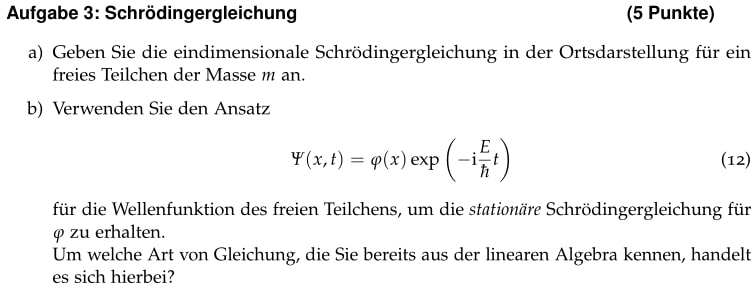
\includegraphics[width=0.75\textwidth]{images/Aufgabe_3ab.jpg}
    \label{fig:3}
\end{figure}

\subsection{a)}

\begin{align}
    \intertext{\flushleft{Die\;}\justifying eindimensionale Schrödingergleichung in der Ortsdarstellung lautet:
    }
    i\hbar \frac{\partial \psi}{\partial t} = - \frac{\hbar^2}{2m} \frac{\partial^2 \psi}{\partial x^2}  + V \psi \label{eq:a}
\end{align}

\subsection{b)}

    \begin{align}
        \Psi(x,t) &= \varphi \cdot e^{-i \frac{E}{\hbar} t}\\
        \frac{\partial \Psi}{\partial t} &= -i \frac{E}{\hbar} \cdot \varphi(x) \cdot e^{-i \frac{E}{\hbar} t} \label{eq:b}\\
        \frac{\partial^2 \Psi}{\partial x^2} &= \frac{\partial^2 \varphi}{\partial x^2} \cdot e^{-i \frac{E}{\hbar} t} \label{eq:c}\\
        \intertext{\flushleft{$e^{-i \frac{E}{\hbar} t} = 1$\;}\justifying, da der stationäre Zustand zeitunabhängig ist. Werden nun Gleichungen \eqref{eq:b} und 
        \eqref{eq:c} in Gleichung \eqref{eq:a} eingesetzt, ergibt sich:
        }\\
        \Rightarrow i \hbar (-i \frac{E}{\hbar} \cdot \varphi(x)) &= - \frac{\hbar^2}{2m} \frac{\partial^2 \varphi}{\partial x^2} + V\varphi \nonumber\\
        \Leftrightarrow E \varphi &= - \frac{\hbar^2}{2m} \frac{\partial^2 \varphi}{\partial x^2} + V\varphi \label{eq:3b}
    \end{align}

    \flushleft{Bei\;}\justifying der Gleichung \eqref{eq:3b} handelt es sich um die Eigenwertgleichung der Energie.


\begin{figure}[H]
    \centering
    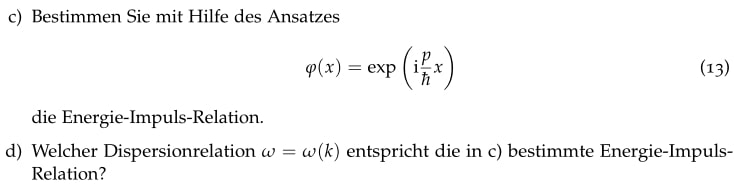
\includegraphics[width=0.75\textwidth]{images/Aufgabe_3cd.jpg}
    \label{fig:4}
\end{figure}

\subsection{c)}

    \begin{align}
        \varphi(x) &= e^{i \frac{p}{\hbar} x}\\
        \frac{\partial^2 \varphi}{\partial x} &= - \frac{p^2}{\hbar^2} \cdot e^{i \frac{p}{\hbar} x}\\
        E &= (- \frac{\hbar}{2m}) \cdot (- \frac{p^2}{\hbar^2}) + V\\
        E &= \frac{p^2}{2m \hbar} + V
    \end{align}

\subsection{d)}

    \begin{align}
        \hbar \omega &= \frac{k^2 \cdot \hbar^2}{2m\hbar} + V \qquad \qquad \text{mit $k = \frac{2\pi}{\lambda}$}\\
        \omega(k) &= \frac{k^2}{2m} + \frac{V}{\hbar} \qquad \qquad \text{mit $p = \frac{2\pi \hbar}{\lambda} = k\hbar$}
    \end{align}

\end{document}